\documentclass[12pt]{article}
\usepackage{fontspec}
\usepackage{polyglossia}
\setmonofont{Courier New}
\setmainlanguage{farsi}
\setotherlanguage{english}
\newfontfamily\persianfont[Script=Arabic]{XBZar}
\usepackage{graphicx}
\usepackage{geometry}
\usepackage{hyperref}
\geometry{a4paper, margin=2.5cm}
\usepackage{setspace}
\usepackage{url}
\onehalfspacing
\usepackage{titling}
\usepackage{float}
\usepackage{etoolbox}
\usepackage[backend=biber,style=numeric,sorting=none]{biblatex}
%%%%%%%%%%%%%%%%%%%%%%%%%%%%%%%%%%%%%%%%%%%%%%%%%%%%%%%%%%%%%%%%%%%%%%%%%%%%%
\makeatletter
\newcommand{\persiandigit}[1]{%
	\ifcase#1 ۰\or ۱\or ۲\or ۳\or ۴\or ۵\or ۶\or ۷\or ۸\or ۹\fi
}
\DeclareFieldFormat{labelnumber}{\persiandigit{#1}}
\makeatother
%%%%%%%%%%%%%%%%%%%%%%%%%%%%%%%%%
\newcommand{\persianordinal}[1]{%
	\ifcase#1
	\or اول%
	\or دوم%
	\or سوم%
	\or چهارم%
	\or پنجم%
	\or ششم%
	\or هفتم%
	\or هشتم%
	\or نهم%
	\or دهم%
	\or یازدهم%
	\or دوازدهم%
	\or سیزدهم%
	\or چهاردهم%
	\or پانزدهم%
	\or شانزدهم%
	\or هفدهم%
	\or هجدهم%
	\or نوزدهم%
	\or بیستم%
	\else #1\fi
}

\newcommand{\persianordinalpage}{\persianfont\persianordinal{\value{page}}}


%%%%%%%%%%%%%%%%%%%%%%%%%%%%%%%%%%%%%%%%%%%%%%%%%%%%%%%%%%%%%%%%%%%%%%%%%%%%%
\begin{filecontents}{\jobname.bib}
	@online{a1,
		url = {https://www.geeksforgeeks.org/c/c-program-demonstrate-fork-and-pipe/}
	}
	@online{a2,
		url = {https://man7.org/linux/man-pages/man7/signal.7.html}
	}
	@online{a3,
		url = {https://man7.org/linux/man-pages/man2/alarm.2.html}
	}
\end{filecontents}

\addbibresource{\jobname.bib}

\defbibheading{bibliography}[]{%
	\begin{RTL}
		\section*{مراجع}
	\end{RTL}
}

%%%%%%%%%%%%%%%%%%%%%%%%%%%%%%%%%%%%%%%%%%%%%%%%%%%%%%%%%%%%%%%%%%%%%%%%%%%%%

\begin{document}
	
	% ==============================
	% Title Page
	% ==============================
	\begin{titlepage}
		\centering
		\vspace*{1cm}
		
\includegraphics[width=4cm]{sharif.png}\\[1.5cm]
		{\Large\textbf{دانشگاه صنعتی شریف}}\\[0.5cm]
		{\large\textbf{دانشکده‌ٔ مهندسی کامپیوتر}}\\[1.5cm]
		{\Huge\textbf{گزارش کار آزمایشگاه}}\\[0.5cm]
		{\LARGE\textbf{آزمایشگاه سیستم‌های عامل}}\\[2cm]
		
		\textbf{گزارش آزمایش شماره ۵}\\
		(ارتباط بین پردازه‌ای)
		
		\vfill
		\begin{tabular}{rl}
			\textbf{شماره‌ی گروه:} & ۲۰ \\
			\textbf{گروه:} &
			ارشیا یوسف‌نیا (۴۰۱۱۱۰۴۱۵) \\
			& محمدعارف زارع زاده (۴۰۱۱۰۶۰۱۷) \\
			\textbf{استاد درس:} & دکتر بیگی \\
			\textbf{تاریخ:} & تابستان ۱۴۰۴ \\
		\end{tabular}
	\end{titlepage}
	
	% ==============================
	% Persian Ordinal Page Numbering
	% ==============================
	\clearpage
	\setcounter{page}{1}
	\renewcommand{\thepage}{\persianordinalpage}
	
	\tableofcontents
	\clearpage
	\listoffigures
	%\clearpage
	%\listoftables
	
	% ==============================
	% Switch to Persian Digits (۱, ۲, ۳, ...)
	% ==============================
	\clearpage
	\setcounter{page}{1}
	\pagenumbering{arabic}
	\renewcommand{\thepage}{\persianfont\arabic{page}}
	
	
	% ==============================
	% Main Content
	% ==============================
	
	\section{ایجاد \textenglish{pipe} یک‌سویه}
	همانطور که در شکل \ref{img:1} آمده مستندات pipe را مطالعه می‌کنیم که برای ارتباط بین‌پردازه‌ای یا \textenglish{IPC (Inter-Process Communication)} به کار می‌رود. در ادامه در شکل \ref{img:2} یک کد حداقلی برای ایجاد یک پایپ یک‌سویه را می‌بینیم. شکل \ref{img:3} هم خروجی را نشان می‌دهد. در این برنامه فقط یک پردازه داشتیم و برای استفاده واقعی باید پردازهٔ فرزند نیز ایجاد کنیم.
	\begin{figure}[H]
		\centering
		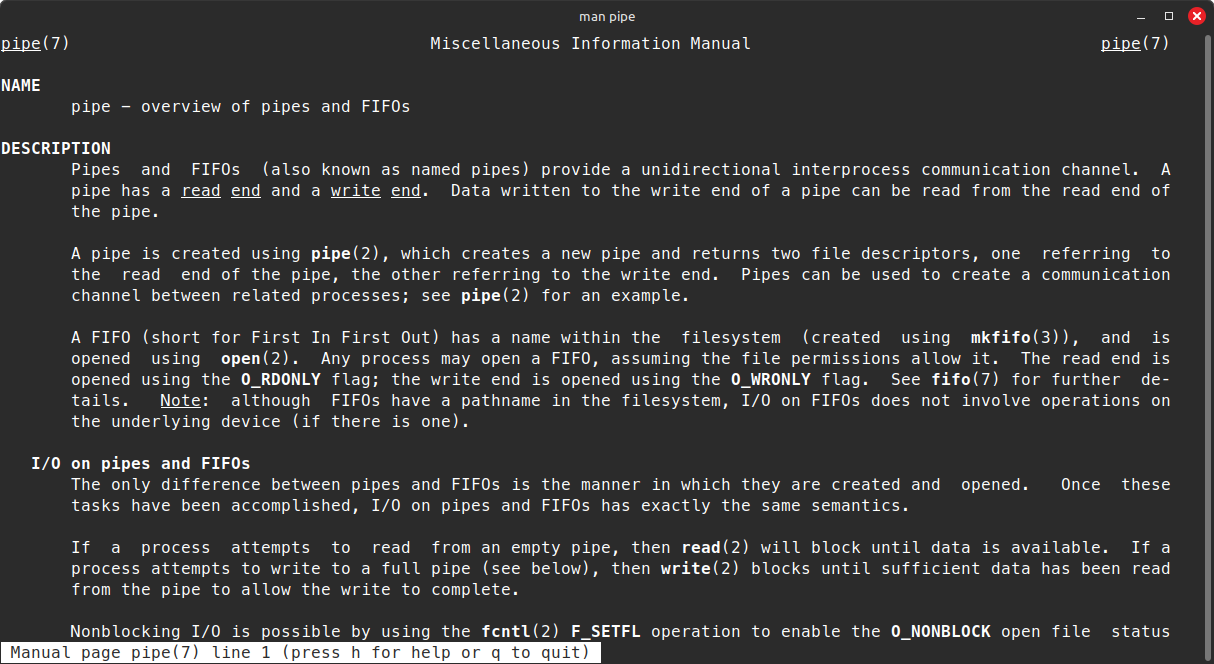
\includegraphics[width=\textwidth]{report5-resources/1.png}
		\caption{توضیحات \textenglish{man pipe}}
		\label{img:1}
	\end{figure}
	\begin{figure}[H]
		\centering
		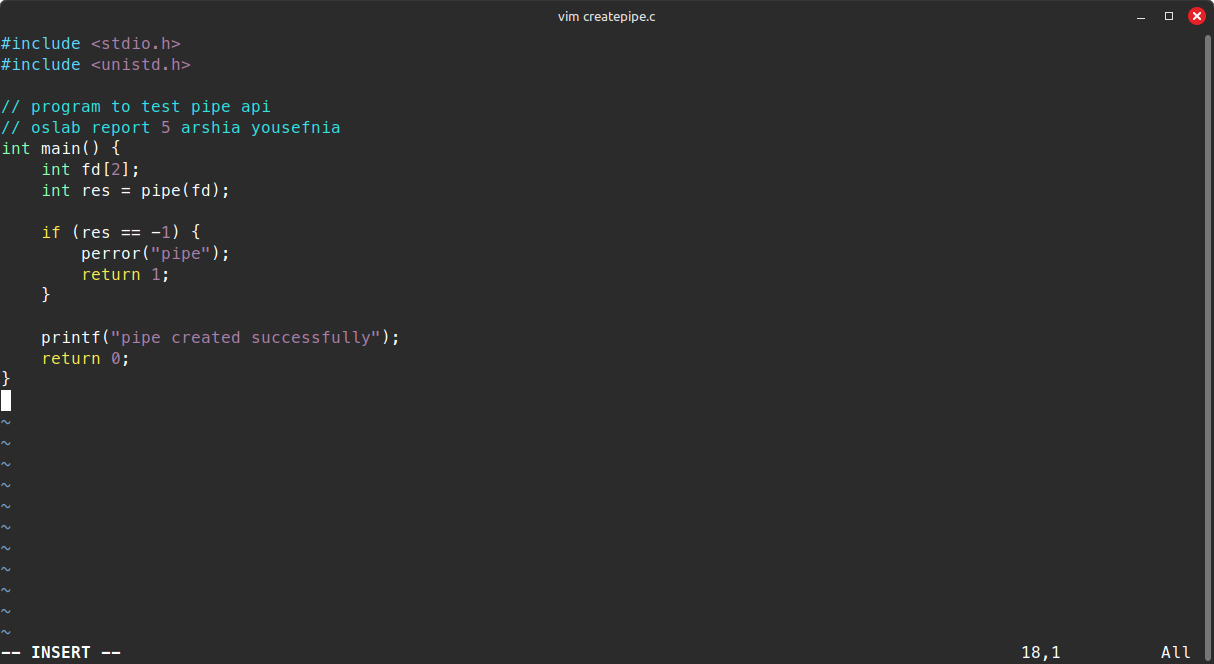
\includegraphics[width=\textwidth]{report5-resources/2.png}
		\caption{برنامهٔ حداقلی برای ساخت موفق یک \textenglish{pipe} یک‌سویه}
		\label{img:2}
	\end{figure}
	\begin{figure}[H]
		\centering
		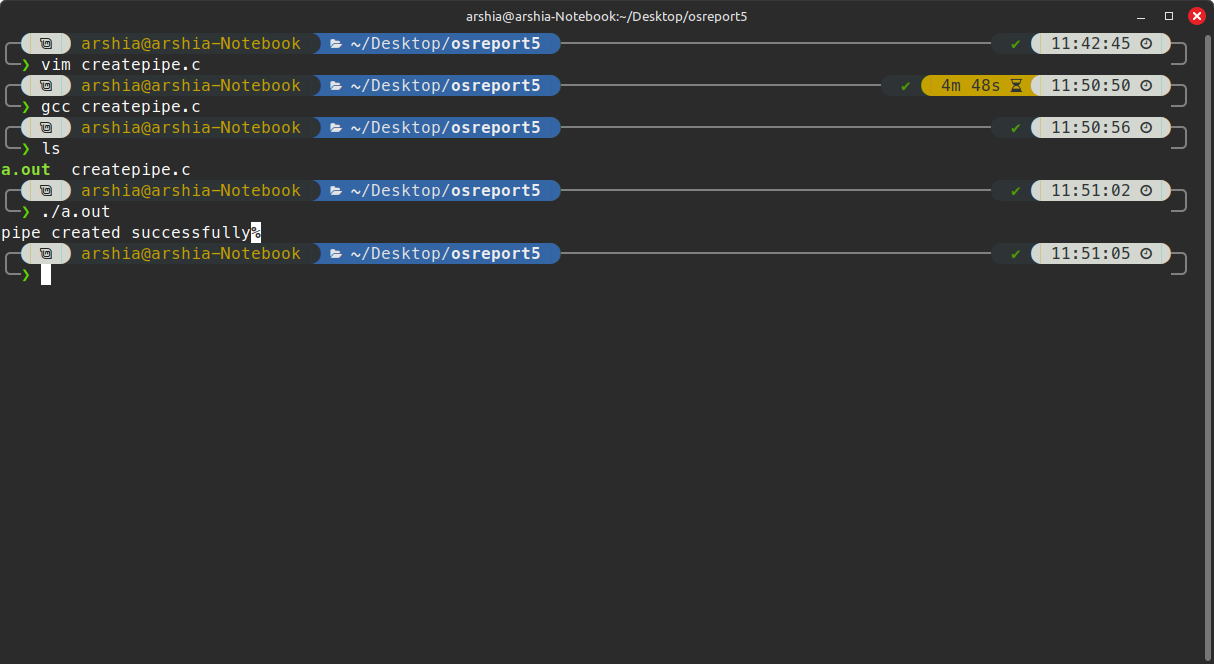
\includegraphics[width=\textwidth]{report5-resources/3.png}
		\caption{مراحل کامپایل و اجرای موفق برنامهٔ شکل \ref{img:2}}
		\label{img:3}
	\end{figure}
	
	در ادامه برای نشان دادن یک کاربرد واقعی، یک پردازهٔ فرزند و یک پایپ درست می‌کنیم. در ادامه یک پیام را از پردازهٔ والد به داخل pipe می‌فرستیم و در پردازهٔ فرزند آن را می‌خوانیم و چاپ می‌کنیم. هر کدام از پردازه‌های والد و فرزند آن \textenglish{File Descriptor} هایی از پایپ را که مربوط به طرف آن‌‌هانیست می‌بندند. این برنامه در شکل \ref{img:4} و نتیجهٔ آن در شکل \ref{img:5} آمده است.
	\begin{figure}[H]
		\centering
		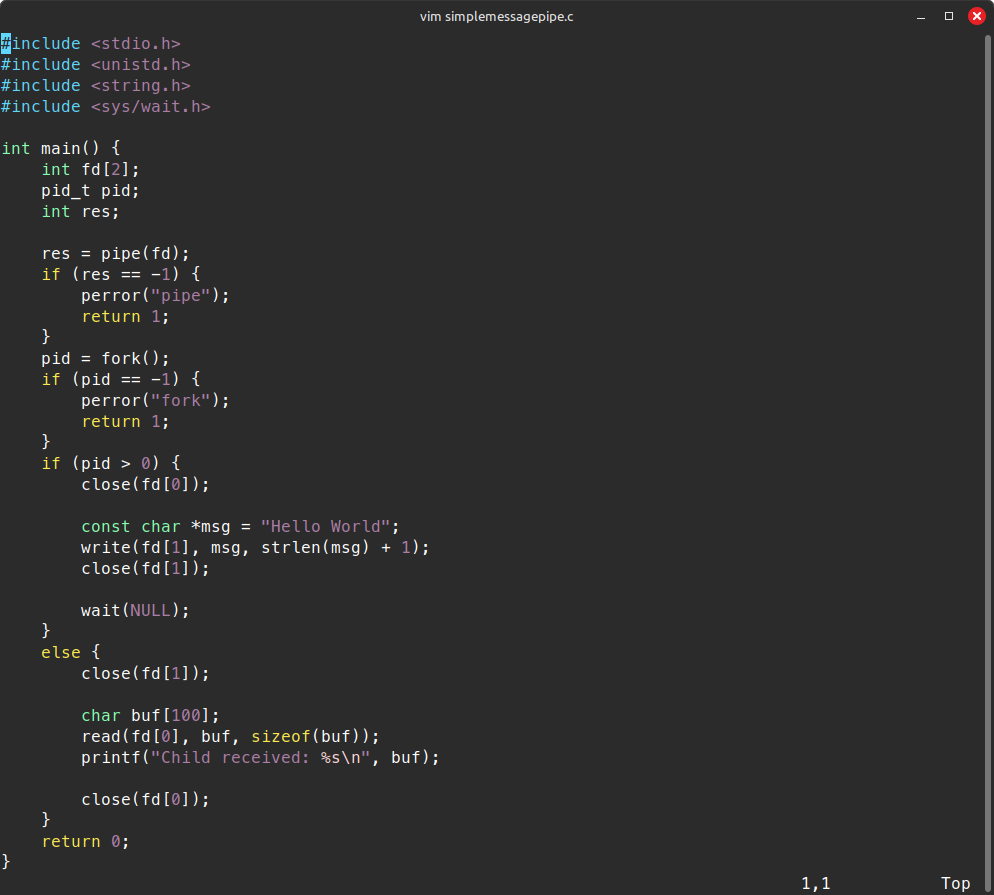
\includegraphics[width=\textwidth]{report5-resources/4.png}
		\caption{برنامهٔ انتقال پیام متنی از پردازهٔ والد به فرزند و چاپ آن در فرزند}
		\label{img:4}
	\end{figure}
	\begin{figure}[H]
		\centering
		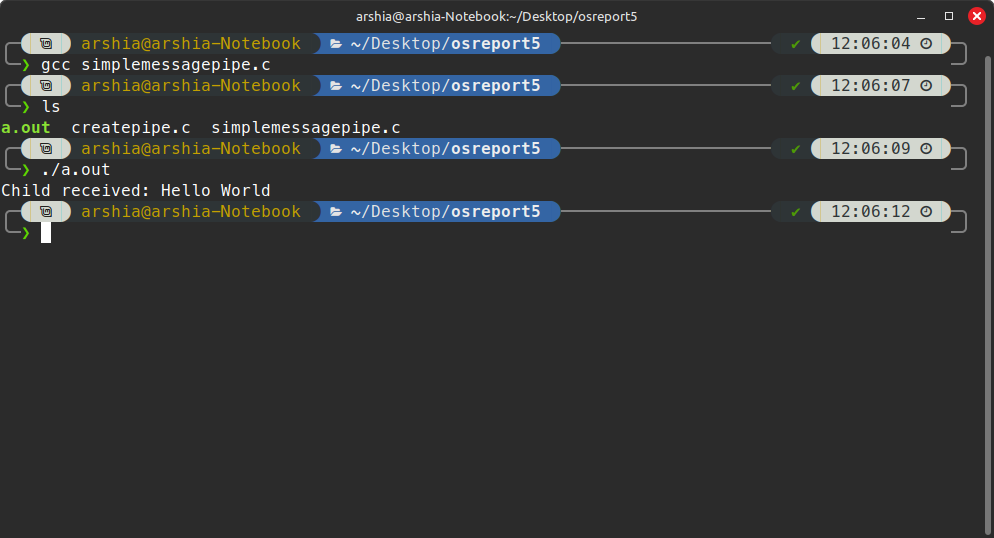
\includegraphics[width=\textwidth]{report5-resources/5.png}
		\caption{مراحل کامپایل و اجرای موفق برنامهٔ شکل \ref{img:4}}
		\label{img:5}
	\end{figure}
	\subsection{فعالیت‌ها}
	در این فعالیت در پردازهٔ والد دستور یا برنامهٔ ls را اجرا می‌کنیم و با یک پایپ آن را به پردازهٔ فرزند می‌فرستیم. پردازهٔ فرزند نیز این منبع را به جای stdin قرار می‌دهد و با آن دستور wc را اجرا می‌کند و خروجی را چاپ می‌کند. با این کار به طور مؤثر پایپ کردن در ترمینال لینوکس را بازسازی می‌کنیم. شکل \ref{img:6} این برنامه را نشان می‌دهد و شکل \ref{img:7} اجرای موفق آن را.
	\begin{figure}[H]
		\centering
		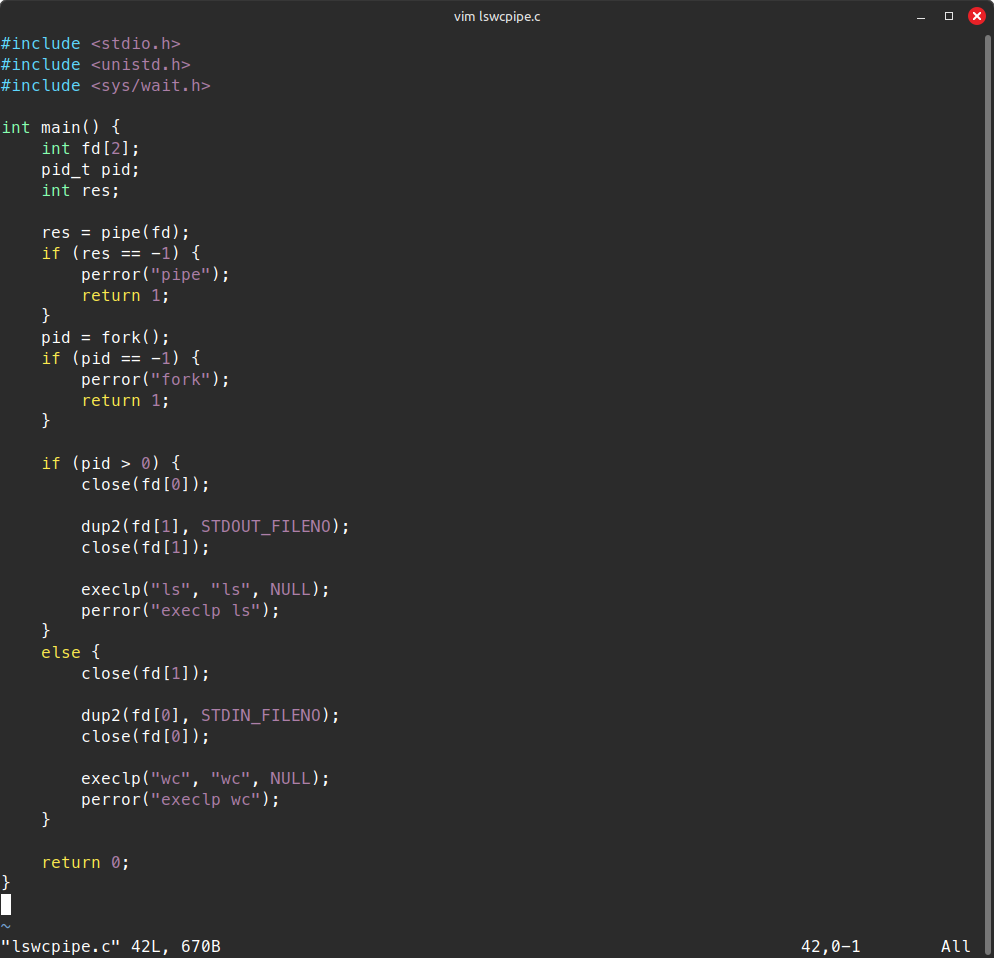
\includegraphics[width=\textwidth]{report5-resources/6.png}
		\caption{برنامهٔ اجرای \textenglish{ls} در پردازهٔ والد و انتقال آن با \textenglish{pipe} به پردازهٔ فرزند و اجرای \textenglish{wc} روی این ورودی و خروجی دادن آن}
		\label{img:6}
	\end{figure}
	\begin{figure}[H]
		\centering
		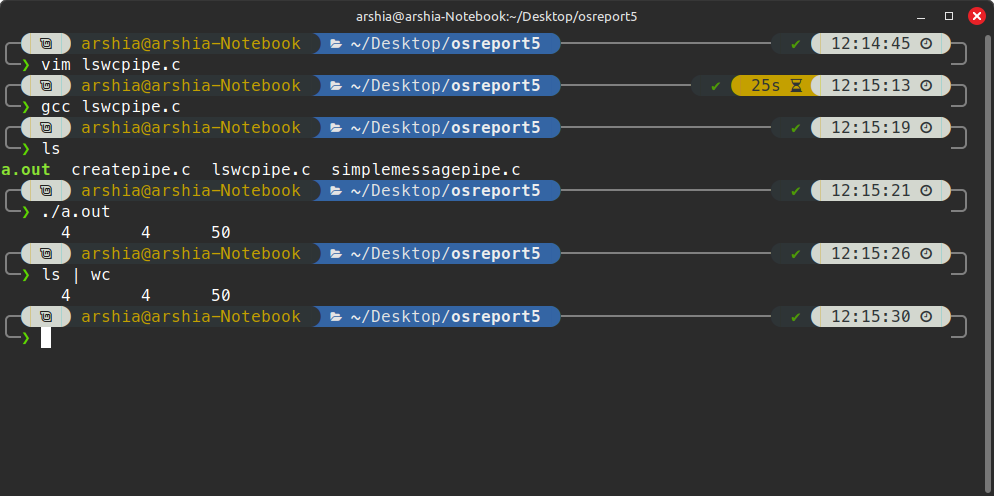
\includegraphics[width=\textwidth]{report5-resources/7.png}
		\caption{مراحل کامپایل و اجرای موفق برنامهٔ شکل \ref{img:6}}
		\label{img:7}
	\end{figure}
	برای ارتباط دوطرفهٔ بین‌پردازه‌ای یک راه منطقی استفاده از دو پایپ یک‌سویه در جهت‌های مختلف است. یک پردازه در یک پایپ می‌نویسد و از آن یکی می‌خواند. برای پردازه مقابل نقش این دو پایپ عوض می‌شود. این روش به خاطر ساختن دو پایپ یک طرفه ساده است \cite{a1}.
	
	\newpage
	\section{سیگنال}
	در شکل \ref{img:8} نمایی از مستندات singal آمده و در شکل \ref{img:9} هم مستندات alarm آمده است.
	
	در ادامه به توضیح تعدادی از سیگنال‌ها می‌پردازیم:
	
	\textenglish{SIGINT	2}
	
		ارسال‌شده وقتی کاربر Ctrl+C می‌زند. معمولاً باعث توقف فرآیند می‌شود.
		
	\textenglish{SIGTERM 15}
	
		سیگنال استاندارد برای پایان دادن به یک فرآیند. برنامه می‌تواند آن را پردازش کند و واکنش مناسبی نشان دهد.
		
	\textenglish{SIGKILL 9}
	
		فرآیند را فوراً و بدون امکان کنترل یا مدیریت متوقف می‌کند. قابل جلوگیری نیست.
		
	\textenglish{SIGSEGV 11}
		
			در صورت تلاش برای دسترسی غیرمجاز به حافظه (مانند اشاره‌گر خراب)، ارسال می‌شود.
			
	\textenglish{SIGALRM 14}
	
		هنگام رسیدن زمان تعیین‌شده توسط \textenglish{alarm()} ارسال می‌شود \cite{a2}.
		
		تابع alarm() برای تنظیم یک تایمر استفاده می‌شود که پس از تعداد مشخصی ثانیه، سیگنال SIGALRM را به فرآیند ارسال می‌کند.
		
		نحوه عملکرد:
		وقتی alarm(seconds) را صدا می‌زنید، سیستم‌عامل یک شمارنده تنظیم می‌کند.
		
		پس از گذشت آن مدت، سیگنال SIGALRM به فرآیند ارسال می‌شود.
		
		اگر برنامه یک handler برای SIGALRM تعریف کرده باشد (با \textenglish{signal(SIGALRM, handler)})، آن تابع اجرا می‌شود.
		
		اگر نه، رفتار پیش‌فرض خاتمه دادن به برنامه است \cite{a3}.
	\begin{figure}[H]
		\centering
		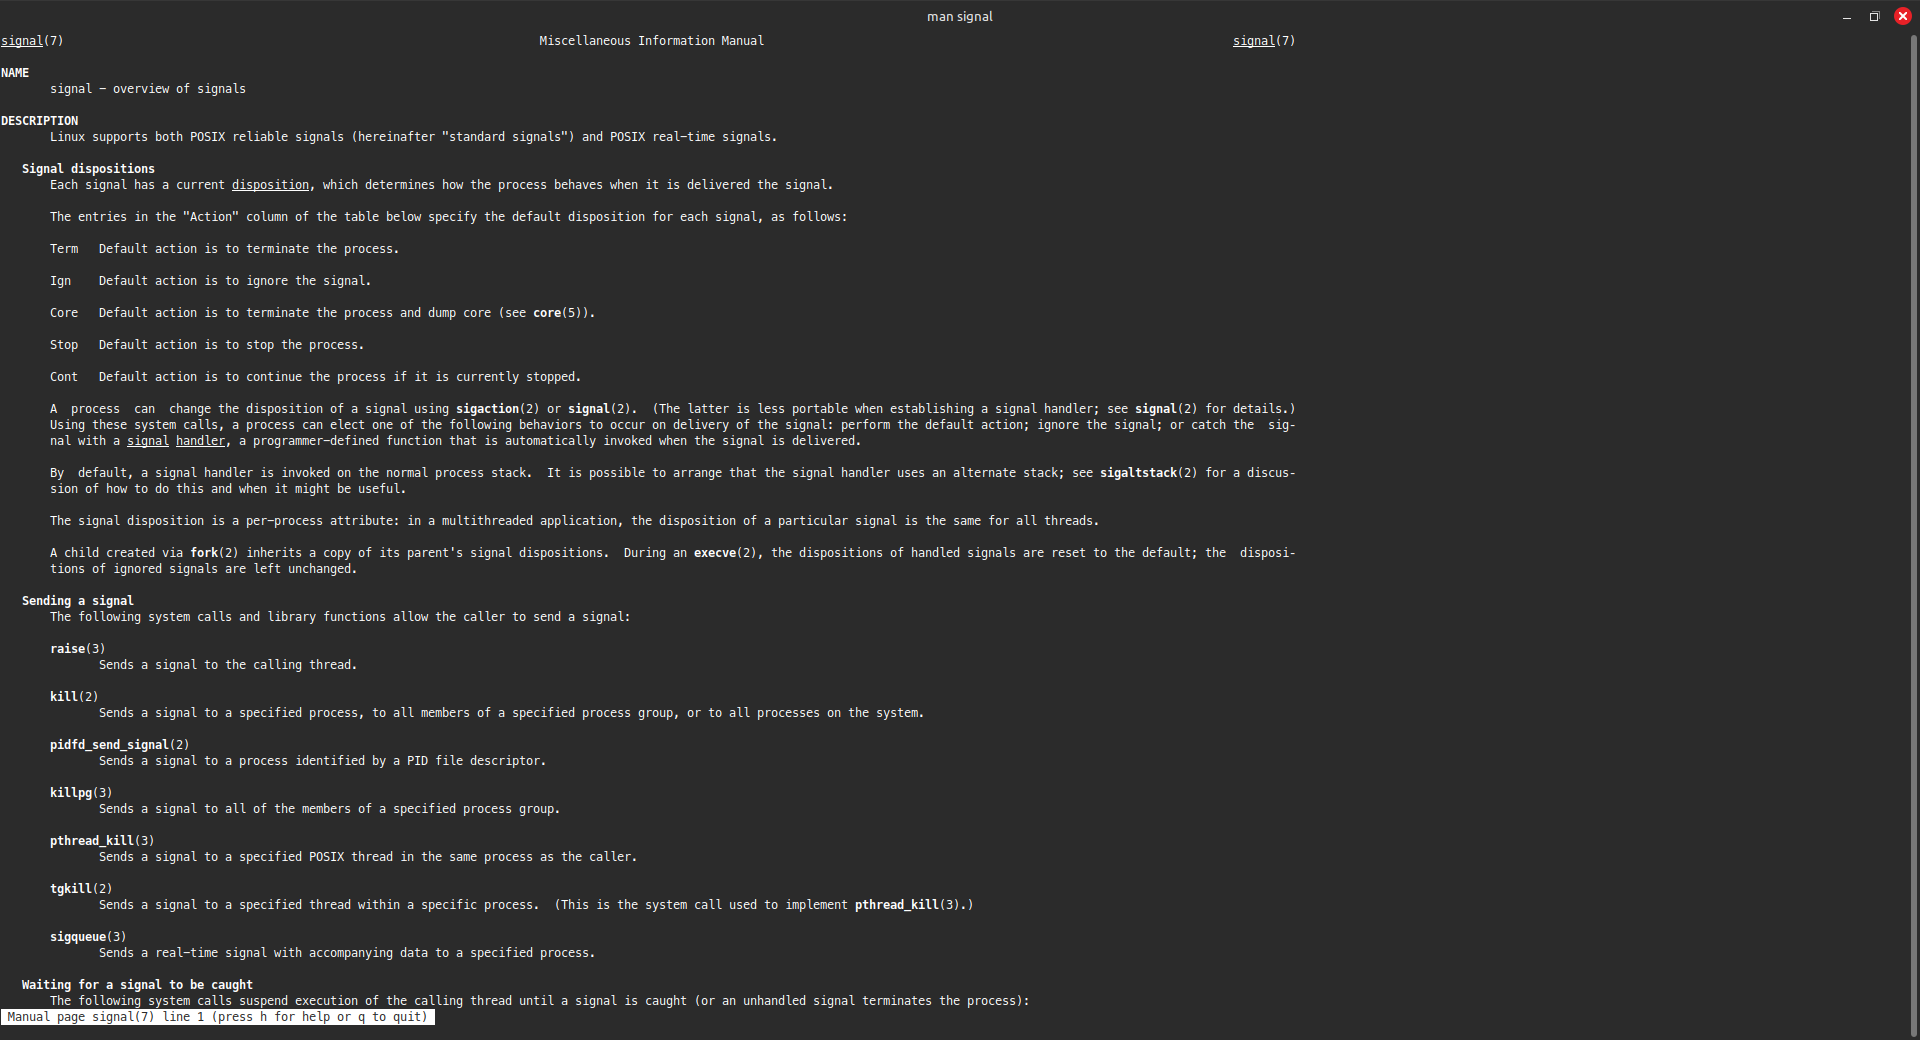
\includegraphics[width=\textwidth]{report5-resources/8.png}
		\caption{توضیحات \textenglish{man signal}}
		\label{img:8}
	\end{figure}
	\begin{figure}[H]
		\centering
		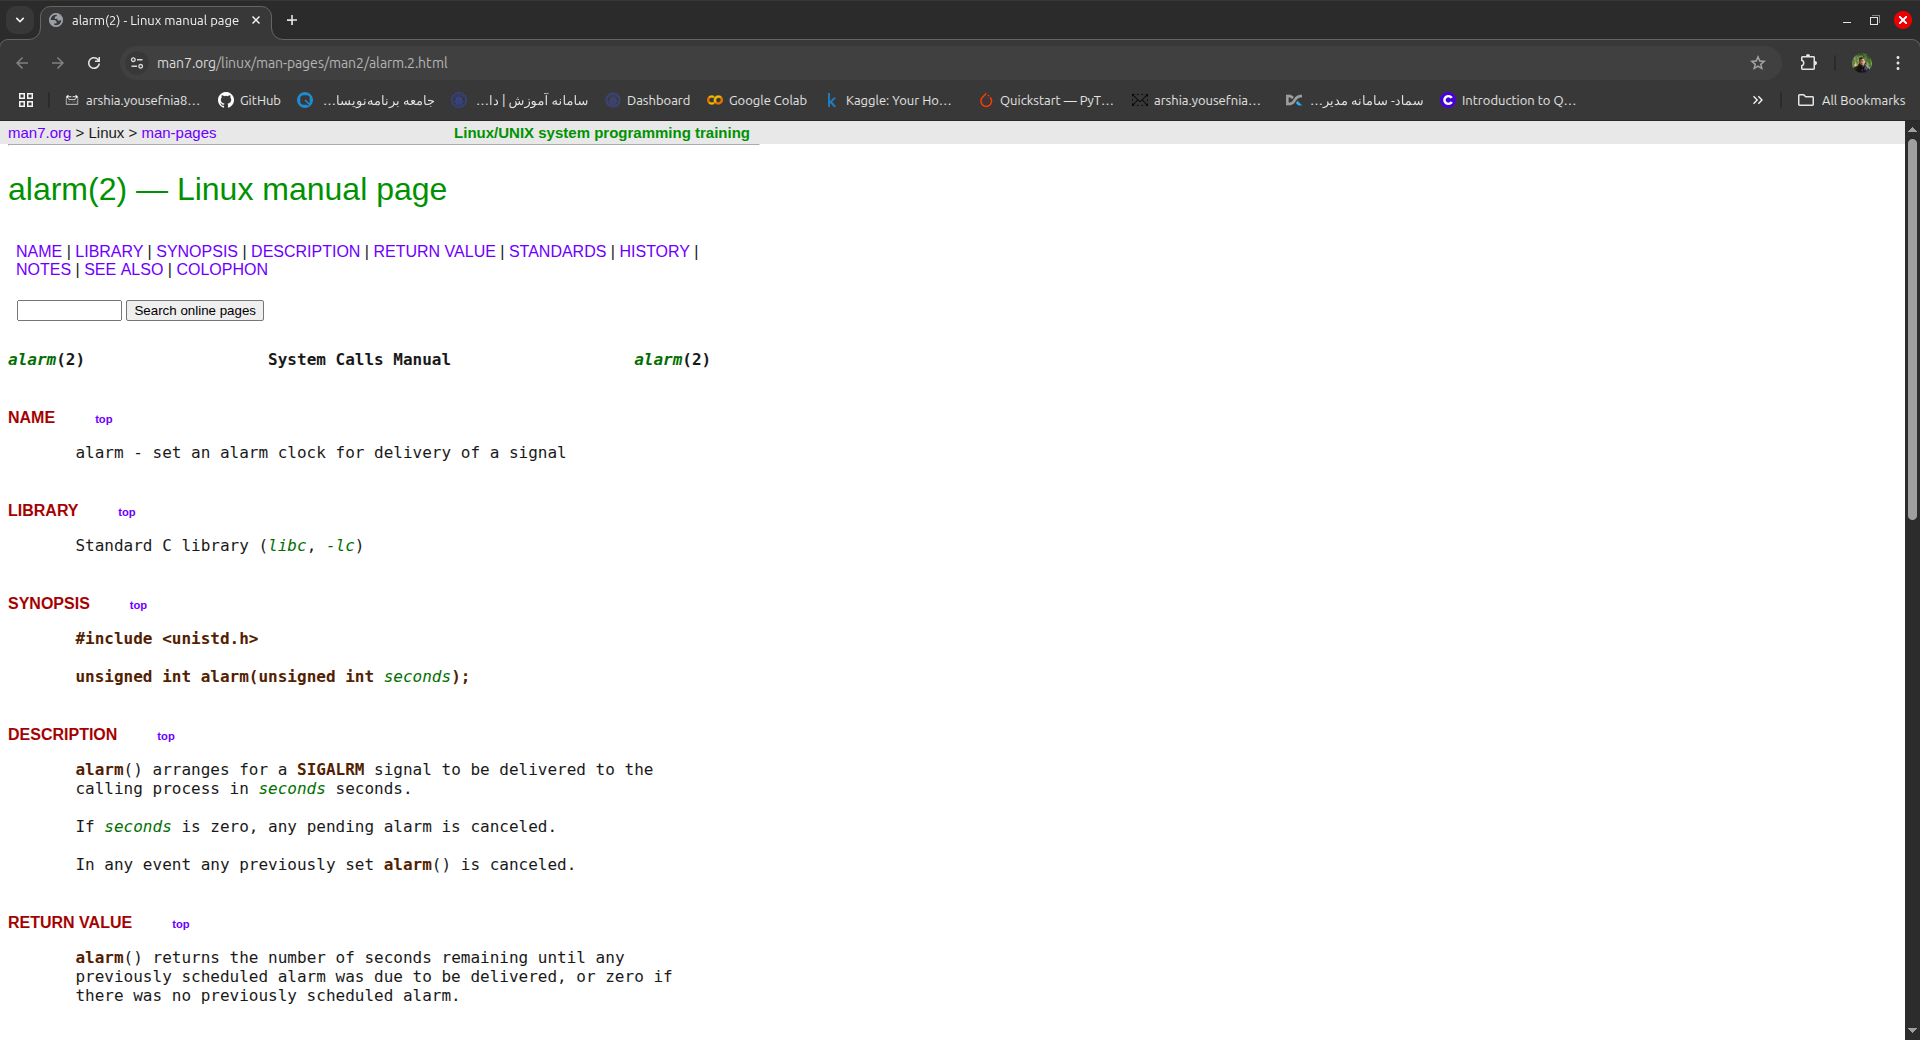
\includegraphics[width=\textwidth]{report5-resources/9.png}
		\caption{صفحه \textenglish{manual} دربارهٔ \textenglish{alarm}}
		\label{img:9}
	\end{figure}
	
	شکل \ref{img:10} برنامهٔ سادهٔ خواسته شده به همراه اجرای آن را نشان می‌دهد. یک آلارم ۵ ثانیه‌ای قرار می‌دهد و یک خط را چاپ می‌کند و سپس در یک حلقه بی‌پایان قرار می‌گیرد و خط آخر را چاپ نمی‌کند. بعد از ۵ ثانیه سیگنال فرستاده می‌شود و برنامه تمام می‌شود.
	\begin{figure}[H]
		\centering
		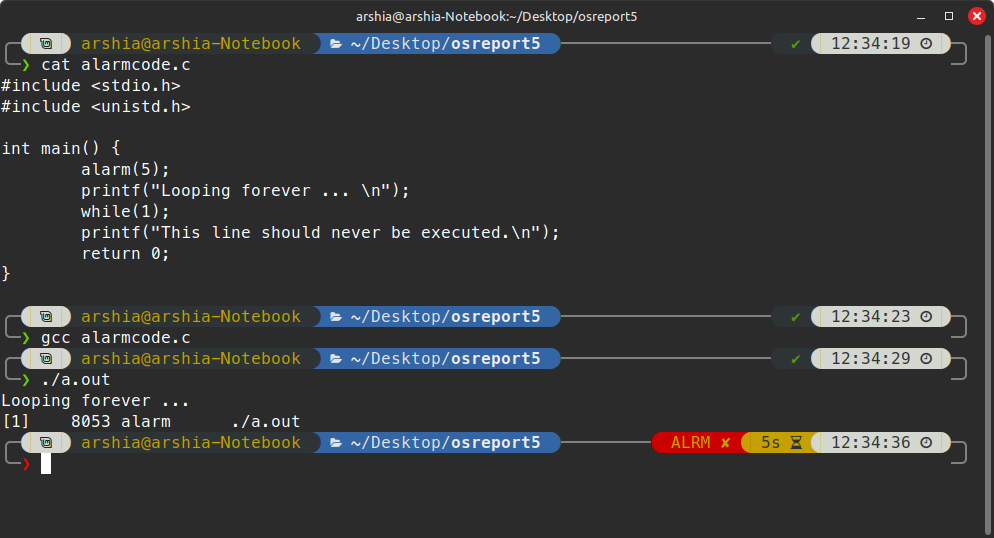
\includegraphics[width=\textwidth]{report5-resources/10.png}
		\caption{استفاده از سیگنال \textenglish{alarm} در یک برنامهٔ ساده به همراه نتیجهٔ اجرا}
		\label{img:10}
	\end{figure}
	شکل \ref{img:11} برنامهٔ تغییر داده شده را نشان می‌دهد. به جای حلقه بی‌پایان برای نگه‌داشتن برنامه در یک جا، از pause برای منتظر یک سیگنال ماندن استفاده می‌کنیم. به علاوه یک handler هم برای این سیگنال اضافه می‌کنیم که رفتار را تغییر دهد و هیچ‌کاری نکند، صرفا یک خط چاپ کند. پس با آمدن سیگنال برنامه ادامه پیدا می‌کند و خط آخر چاپ می‌شود. شکل \ref{img:12} مراحل اجرای این برنامه را نشان می‌دهد.
	\begin{figure}[H]
		\centering
		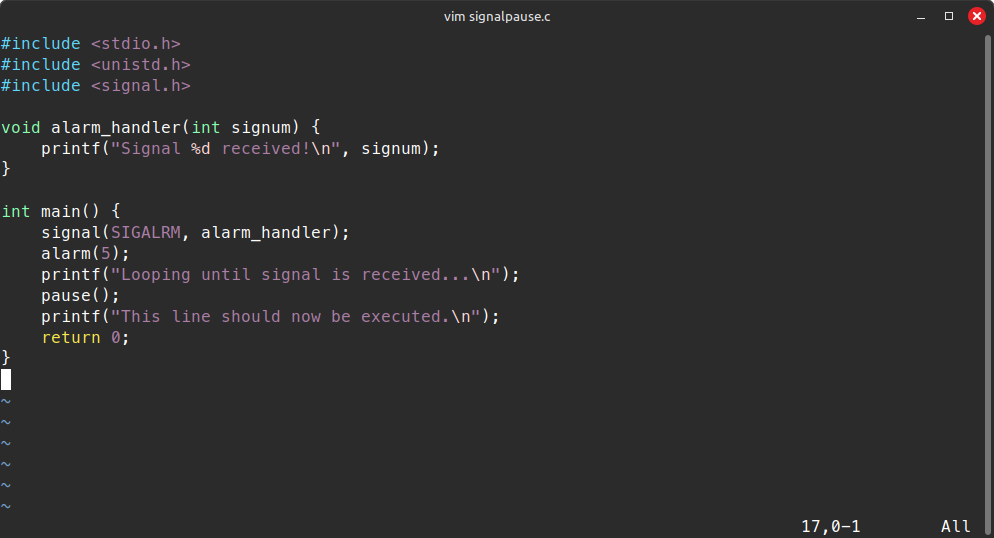
\includegraphics[width=\textwidth]{report5-resources/11.png}
		\caption{تغییر برنامهٔ شکل \ref{img:10} با \textenglish{signal} و \textenglish{pause} برای کارایی خواسته شده}
		\label{img:11}
	\end{figure}
	\begin{figure}[H]
		\centering
		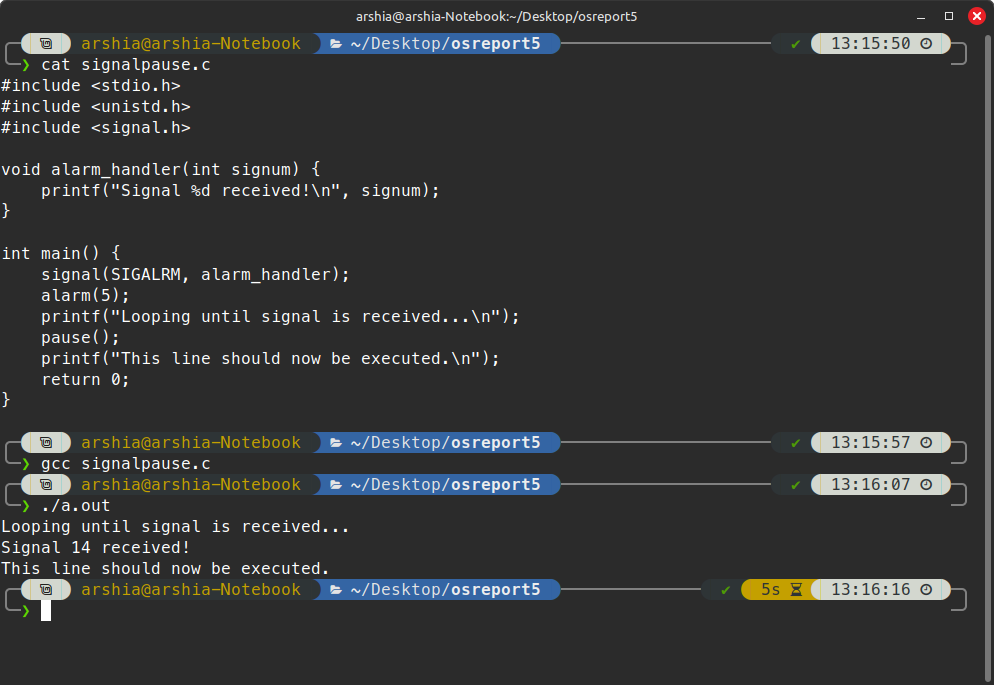
\includegraphics[width=\textwidth]{report5-resources/12.png}
		\caption{مراحل کامپایل و اجرای برنامهٔ شکل \ref{img:11}}
		\label{img:12}
	\end{figure}
	\subsection{تمرین}
	در این تمرین با دانش قسمت قبل، یک برنامه می‌نویسیم که در واکنش به سیگنال ارسالی از \textenglish{CTRL+C} در بار اول متوقف نشود، ولی با بار دوم برنامه تمام شود. واضحا باید یک handler مناسب اضافه کنیم و به تعداد زیاد pause درست کنیم. این کار با قرار دادن pause در حلقهٔ بی‌پایان انجام می‌شود. برنامه در شکل \ref{img:13} آمده است. در شکل \ref{img:14} هم نتیجهٔ اجرا آمده است.
	\begin{figure}[H]
		\centering
		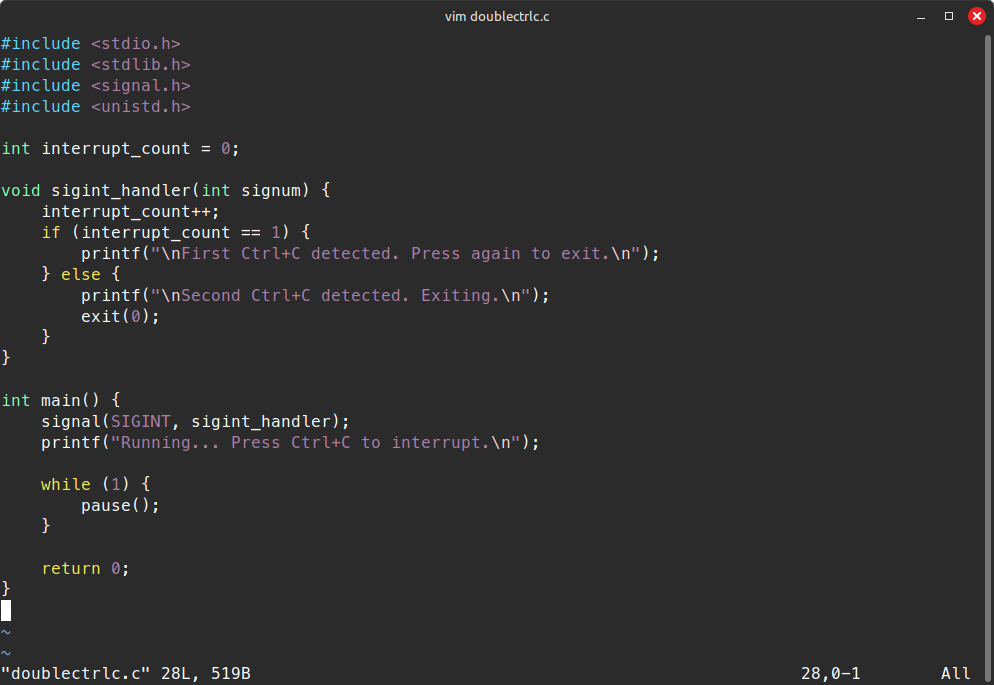
\includegraphics[width=\textwidth]{report5-resources/13.png}
		\caption{برنامهٔ حداقلی برای خروج از برنامه با دوبار \textenglish{CTRL+C} به جای پیشفرض یک‌بار}
		\label{img:13}
	\end{figure}
	\begin{figure}[H]
		\centering
		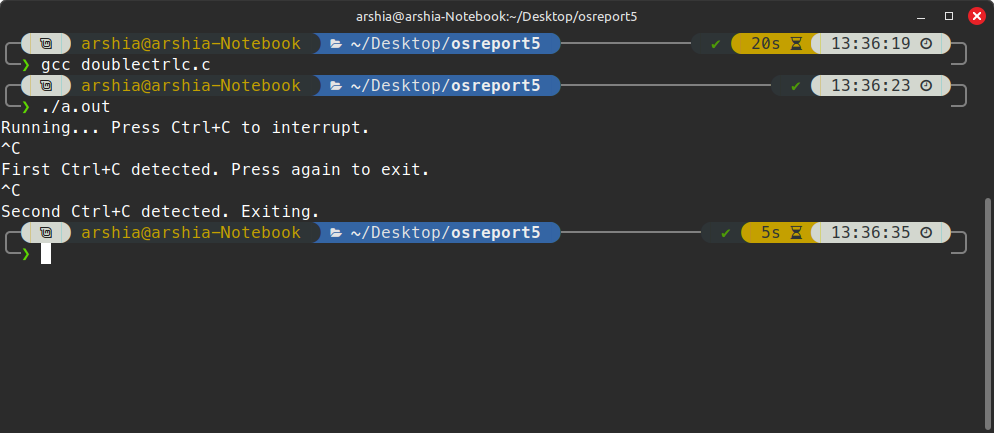
\includegraphics[width=\textwidth]{report5-resources/14.png}
		\caption{مراحل کامپایل و اجرای برنامهٔ شکل \ref{img:13}}
		\label{img:14}
	\end{figure}
        
	% ==============================
	% References
	% ==============================
	\newpage
	\begin{LTR}
		\printbibliography[title={مراجع}]
	\end{LTR}

	
\end{document}

